\chapter{Исследовательская часть}

\section{Технические характеристики}

Технические характеристики устройства, на котором выполнялось тестирование:

\begin{itemize}
	\item Операционная система: Ubuntu\cite{ubuntu} Linux x86\_64.
	\item Память: 16 GiB.
	\item Процессор: AMD Ryzen™ 7 4700U\cite{amd}.
\end{itemize}

\section{Время выполнения алгоритмов}

Тестирование проводилось на ноутбуке, включенном в сеть электропитания. Во время тестирования ноутбук был нагружен только встроенными
приложениями окружения, окружением, а также непосредственно системой тестирования.

\section{Время выполнения алгоритмов}

Алгоритмы тестировались при помощи встроенного встроенного модуля \texttt{timeit}\cite{timeit}. Специальная функция делает 50 замеров и в качестве результата возвращает среднее значение.

Результаты замеров приведены в таблице \ref{tbl:profilingalgs} В данной таблице для значений, для которых тестирование не выполнялось, в поле результата находится $NaN$. На рисунках \ref{img:profiling1} и \ref{img:profiling2} приведены графики зависимостей времени работы алгоритмов от длины строк.

\begin{table} [h!]
	\caption{Таблица времени выполнения алгоритмов (мс)}
	\label{tbl:profilingalgs}
	\begin{center}
		\begin{tabular}{|c|c|c|c|c|} 
		 	\hline
			Длина строк & LevRec & DamLevRec & LevRecMem & DamLevMatrix \\  
		 	\hline
		 	3 & 3.591 & 3.784 & NaN & NaN\\
		 	\hline
		 	5 & 573.876 & 428.998 & NaN & NaN\\
		 	\hline
		 	7 & 16357.543 & 20189.442 & NaN & NaN\\
		 	\hline
		 	10 & 1434103.206 & 3197884.986 & 95.161  & 59.505 \\
		 	\hline
		 	50 & NaN & NaN & 2285.094 &  1374.323 \\
		 	\hline
		 	100 & NaN & NaN & 9420.838 & 5464.0038 \\
		 	\hline
			200 & NaN & NaN & 37634.303 & 21797.016 \\
			\hline
			300 & NaN & NaN & 87196.739 & 50530.042  \\
			\hline
			400 & NaN & NaN & 166520.663 & 94606.463 \\
			\hline
			500 & NaN & NaN & 258407.907 & 149814.719 \\
			\hline
		\end{tabular}
	\end{center}
\end{table}

\begin{figure}[h]
	\centering
	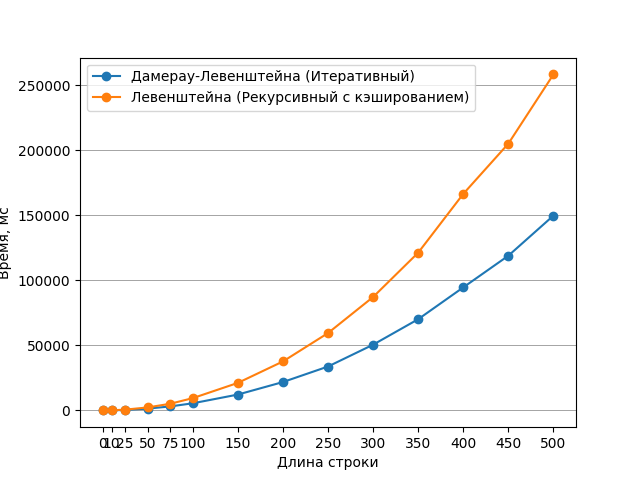
\includegraphics[scale=0.4]{imgs/2.png}
	\caption{Зависимость времени работы алгоритма вычисления
расстояния Левенштейна (рекурсивный с кэшированием) и Дамерау-Левенштейна (итеративный) от длины строк}
	\label{img:profiling1}
\end{figure}

\begin{figure}[h]
	\centering
	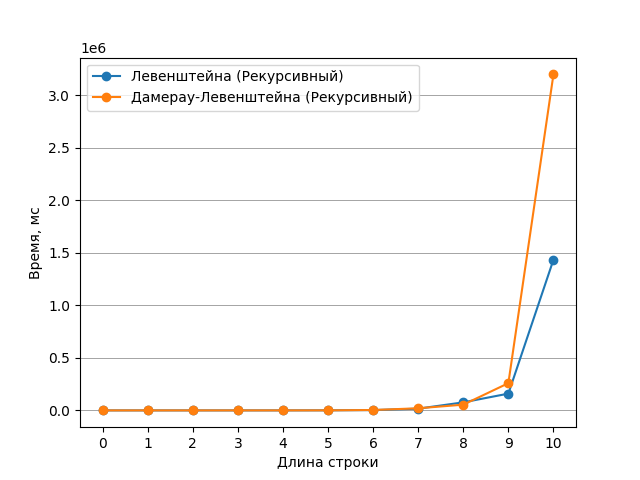
\includegraphics[scale=0.4]{imgs/1.png}
	\caption{Зависимость времени работы алгоритма вычисления
расстояния Левенштейна (рекурсивный) и Дамерау-Левенштейна (рекурсивный) от длины строк}
	\label{img:profiling2}
\end{figure}


\section{Использование памяти}

Алгоритмы нахождения расстояний Левенштейна и Дамерау—Левенштейна не отличаются друг от друга с точки зрения использования памяти, следовательно, достаточно рассмотреть лишь разницу рекурсивной и матричной реализаций этих алгоритмов.

Максимальная глубина стека вызовов при рекурсивной реализации равна сумме длин входящих строк, при этом для каждого вызова рекурсии в моей реализации требуется:

\begin{itemize}
    \item 2 аргумента типа строка: $2 \cdot size(str) = 2 \cdot 44 = 88$ байт (примерно);
    \item 2 локальные переменные типа $int$, в моем случае: $2 \cdot 4 = 8$ байт;
    \item адрес возврата: 8 байт;
    \item место для записи возвращаемого функцией значения: 8 байт.
\end{itemize}
Таким образом получается, что при обычной рекурсии на один вызов требуется (\ref{for:onecall}): 

\begin{equation}
M_{per call} = 88 + 8 + 8 + 8 = 112 \text{ байта}
\label{for:onecall}
\end{equation}

Следовательно память, расходуемая в момент, когда стек вызовов максимален, равна (\ref{for:rec}): 

\begin{equation}
    M_{recursive} = 112 \cdot depth
\label{for:rec}
\end{equation}

где \textit{depth} - максимальная глубина стека вызовов, которая равна (\ref{for:depth}):

\begin{equation}
depth = |S_1| + |S_2|
\label{for:depth}
\end{equation}

где $S_1, S_2$ - строки.

Если мы используем рекурсивный алгоритм с заполнением матрицы матрицы, то для каждого вызова рекурсии добавляется новый аргумент - ссылка на матрицу размером $8$ байт. Также в данном алгоритме требуется память на саму матрицу, размеры которой: $m = |S_1| + 1, n = |S_2| + 1$. Размер элемента матрицы равен размеру $int$, используемого в моей реализации, то есть $4$ байт. Отсюда выходит, что память, которая тратится на хранение матрицы (\ref{for:matrix}):
\begin{equation}
M_{Matrix} = (|S_1| + 1) \cdot (|S_2| + 1) \cdot 4 + 8
\label{for:matrix}
\end{equation}

Таким образом, при рекурсивной реализации требуемая память равна (\ref{for:rec_mem}):
\begin{equation}
M_{recursive} = 112 \cdot depth + M_{Matrix}
\label{for:rec_mem}
\end{equation}
где $M_{Matrix}$ взято из соотношения \ref{for:matrix}.

Память, требуемая для при итеративной реализации, состоит из следующего:
\begin{itemize}
    \item 2 локальные перeменные типа $int$, в моем случае: $2 \cdot 4 = 8$ байт;
    \item 2 аргумента типа строка: $2 \cdot 44 = 88$ байта;
    \item адрес возврата: 8 байт;
    \item место для записи возвращаемого функцией значения: 4 байт;
    \item матрица: $M_{Matrix}$ из соотношения \ref{for:matrix}.
\end{itemize}

Таким образом общая расходуемая память итеративных алгоритмов (\ref{for:iter}):

\begin{equation}
M_{iter} = M_{Matrix} + 108
\label{for:iter}
\end{equation}

где $M_{Matrix}$ определяется из соотношения \ref{for:matrix}.

\section{Вывод}

Рекурсивный алгоритм нахождения расстояния Левенштейна работает
на порядок дольше итеративных реализаций, время его работы увеличивается в геометрической прогрессии. На словах длиной 10 символов, матричная реализация алгоритма нахождения расстояния Левенштейна превосходит по времени работы рекурсивную на несколько порядков.

Алгоритм нахождения расстояния Дамерау—Левенштейна по времени выполнения сопоставим с алгоритмом нахождения расстояния Левенштейна. В нём добавлена дополнительная проверка, позволяющая находить ошибки пользователя, связанные с неверным порядком букв, в связи с чем он работает незначительно дольше, чем алгоритм нахождения расстояния Левенштейна.
    
В то же время по расходу памяти итеративный алгоритмы проигрывает рекурсивному: максимальный размер используемой памяти в них растёт как произведение длин строк (необходимость хранить матрицу), в то время как у рекурсивного алгоритма — как сумма длин строк. Рекурсивный алгоритм с заполнением матрицы превосходит простой рекурсивный и сравним по времени работы с матричными алгоритмами
